%!TEX root = ../thesis.tex

\chapter[discussion]{Discussion}\label{chp:discussion}
% ~5 pages
%
% OUTLINE:
% - paper-hierarchical:
%   - Suitability of VAEs for representation learning (minimization of mutual information and sensitivity to implicit prior such as architecture)
% - paper-benchmarking
%   - Inferiority of probabilistic methods compared to self"=supervised learning. 
% - 

During the three years since the start of this project, the rapid development of machine learning that started about a decade ago with the 2012 ImageNet competation and the work of \textcite{krizhevsky_imagenet_2012} all but slowed down. 
In this section we will briefly revisit selected chapters of the thesis and provide some additional thoughts and discussion. 


\section{Speech representations and uncertainty}
%
In this thesis we have studied two different approaches to learning speech representations: VAEs in \cref{chp:paper-hierarchical,chp:paper-modelagnostic,chp:paper-benchmarking} and self"=supervised methods in \cref{chp:paper-review}. 
We found that the probabilistic formulation of VAEs provide benefits for their application to uncertainty quantification but that they are generally inferior to self"=supervised methods when it comes to performance on downstream tasks, such as phoneme recognition (see e.g. \cref{tab: phoneme recognition (PER), tab:unsupervisedASR}). 
Considering VAEs and self"=supervised methods, it seems we cannot build a model that has a principled probabilistic representation of uncertainty without sacrificing some of the ability to learn rich representations that are useful for downstream applications. 




% VAEs are good at uncertainty quantification (let's at least say that they are).
% SSL methods are very good at representation learning as reflected by their dominance on downstream task performance in for text and speech. 





\subsection{Improved representation learning with variational autoencoders}

One way to improve the representations learned in VAEs is via semi-supervised learning. 
Here a small number of labels are used to inform which patterns that are learned from a large, mostly unlabelled, data set. 
This is usually done by defining a new stochastic variable as the target and deriving a semi-supervised version of the ELBO that accomadates using the labels when they are available, or marginalizing the target variable when they are not. The VAE is then trained on the labelled and unlabelled data simultanously. 

VAEs are strong models for semi-supervised learning as proven in several works \parencite{kingma_semi-supervised_2014,kingma_improved_2016,maaloe_biva_2019}. 
However, self"=supervised methods methods have established themselves as superior also in this setting \cite{jiang_speech_2021, liu_learning_2023}. 
Furthermore, by training on labelled and unlabelled data simultaneously, the semi-supervised setting of VAEs is more constraining than it is for self-supervised methods that divide the training into pre"=training and finetuning. Here, expensive pre"=training yields a single foundation model that can be fine"=tuned at relatively low cost for a large number of downstream tasks, while VAEs must learn all relevant downstream tasks while also learning from the unlabelled data, which is more expensive, but also requires retraining on the unlabelled data, when a . 


Masking in variational autoencoders

Masked pre"=trained as maximum likelihood



\subsection{Uncertainty estimation with self-supervised methods}
%

\textcite{pasad_layerwise_2021} found that layers 6-7 hold the most information about phonetic content and word identity and meaning for \texttt{wav2vec2-base}. 
For \texttt{wav2vec2-large} the phonetic content is highest in layers 11 and 18-19 with a drop in between, while word identity and meaning are highest between layers 12 and 18. 







\section{\Cref{chp:paper-hierarchical} revisited: \dots}

\lesstodo[inline]{Discuss sensitivity to ``implicit" prior such as architecture (and probably optimization method and other). Include reference to \parencite{huszar_is_2017} discussing the usefulness of using a maximum likelihood objective for representation learning in generative models.}
\lesstodo[inline]{Discuss whether VAEs are even suitable for representation learning due to them minimizing a mutual information term in the ELBO (derive this form).}
\lesstodo[inline]{Discuss some recent work e.g. \cref{morningstar_density_2021}}


\section{\Cref{chp:paper-benchmarking} revisited: Bested?}

\lesstodo[inline]{Discuss whether variational autoencoders are viable for learning good representations for speech for downstream tasks when alternatives such as SSL method exist.}
\lesstodo[inline]{Out-of-distribution detection on speech?}


\section{\Cref{chp:paper-review} revisited: \dots} \label{sec:discussion-paper-review}

\lesstodo[inline]{Are self"=supervised speech representations useful for unsupervised uncertainty estimation? \parencite{nava_stateconsistency_2021, nava_uncertaintyaware_2021} Within robotics but not really related.}
% Since the main focus within self"=supervised learning has been on improving downstream task performance, very limited work, if any, has investigated self"=supervised representations in terms of uncertainty estimation. 
% However, in the context of medical applications where data can be abundant but labels are sparse, unsupervised uncertainty estimation is a very interesting direction for future work.
\lesstodo[inline]{OOD data: Generalization or detection (https://arxiv.org/pdf/2110.11334.pdf)?}


\section{\Cref{chp:paper-retrospective} revisited: Calibration}
Our work on stroke recognition in \cref{chp:paper-retrospective} focuses on the predictive performance of the ensemble model and an analysis of feature importance, but does not explicitly consider uncertainty estimation. 
As we discussed in \cref{subsec:model-calibration}, such a model can be calibrated to predict probabilities that are aligned with the empirical probability of the model being correct on some validation set. Here we present and discuss model calibration for the ensemble model. 

We compute the calibration curve by sorting the probabilities predicted on the test set into a number of bins spanning the range from zero to one. For each bin $b$, we compute the mean predicted probability $\bar{p}$ and the fraction of examples for which the model predicted correctly $r_{b}$. The calibration curve is the drawn from the $\{(\bar{p}_{b}, r_{b})\}_b$ pairs. A perfectly calibrated model would have the same fraction of correct predictions in any given bin, as that bin's mean value, $\bar{p}_{b} = r_{b}\,\forall\,b$. 

The calibration curve for the uncalibrated stroke recognition ensemble and its constituent models is plotted in \cref{fig_discussion:retrospective-paper-calibration-curve-of-uncalibrated-model} along with a histogram of its predicted probabilities. The miscalibration issue that we previously discussed is clearly visible as a strong overconfidence. 
Additionally, the ensemble model is appreciably better calibrated than its constituent models. Since the ensemble output probability is computed as the harmonic mean of the five constituent model probabilities, the ensemble's output probability can never exceed the maximum probability predicted between the constituent models. This property tends to make ensemble probabilities less extreme and, since the constituent models are overconfident, this results in better calibration (see also the histogram in \cref{fig_discussion:retrospective-paper-calibration-curve-of-uncalibrated-model}). 

\begin{figure}
    \begin{subfigure}[c]{0.48\columnwidth}
        \centering
        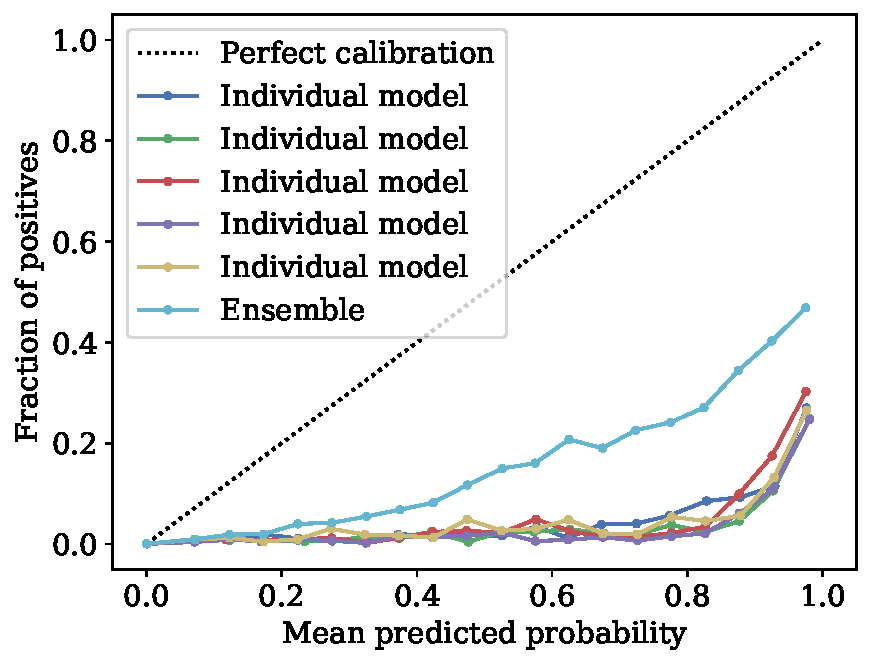
\includegraphics[width=1\columnwidth]{paper_retrospective_calibration_plots/calibration_curve_ensemble_and_all_models_uncalibrated.pdf}
        % \caption{}
        % \label{fig_discussion:calibration_curve_ensemble_and_all_models_uncalibrated}
    \end{subfigure}
    % \hfill
    \begin{subfigure}[c]{0.48\columnwidth}
        \centering
        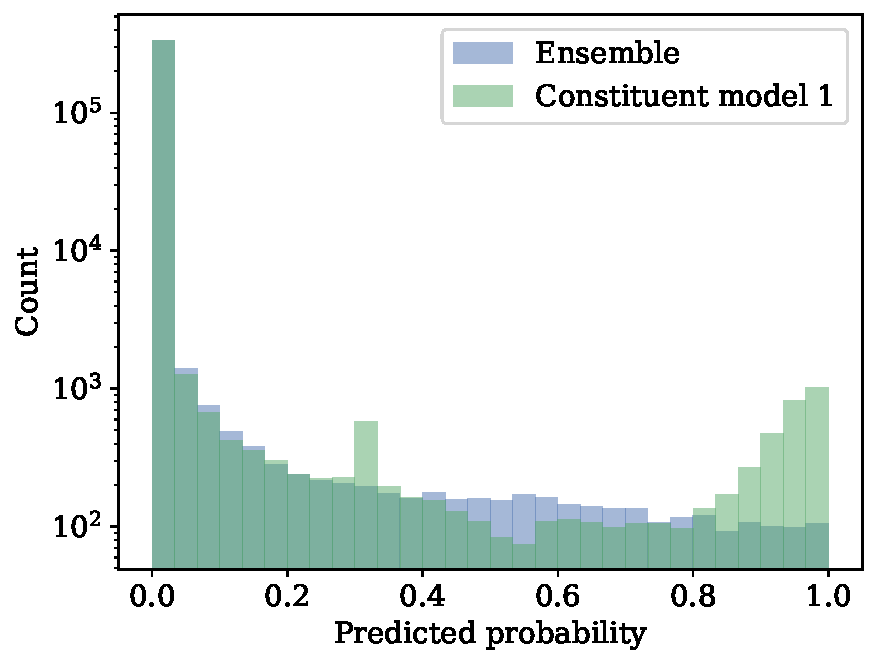
\includegraphics[width=1\columnwidth]{paper_retrospective_calibration_plots/histogram_ensemble_and_single_model.pdf}
        % \caption{}
        % \label{fig_discussion:histogram_ensemble_and_single_model}
    \end{subfigure}
    \caption[Calibration curve for the uncalibrated stroke recognition ensemble and empirical distribution of predicted probabilities.]{%
        Calibration curve for the uncalibrated stroke recognition ensemble (left) and the histogram of predicted probabilities (right) for the test set. 
        We use the ensemble that achieved the median F1-score reported in \cref{tab_retrospective:table3-occlusion-analysis} and \cref{fig_retrospective:figure1-roc-curve}.}
    \label{fig_discussion:retrospective-paper-calibration-curve-of-uncalibrated-model}
\end{figure}

To calibrate the ensemble model, we can use methods such as Platt-scaling \parencite{platt_probabilistic_1999} or isotonic regression \parencite{zadrozny_transforming_2002}. 
We fit a simple regression model (logistic or isotonic) to the predicted probabilities and the target labels on the validation set and use it to adjust the probabilities predicted on the test set. We show the resulting calibration curves on the left in \cref{fig_discussion:retrospective-paper-calibration-curve-sigmoid-isotonic} and the logistic and isotonic fits on the right. 
% In \cref{fig_discussion:retrospective-paper-calibration-curve-sigmoid-isotonic} we have done so for the ensemble model and visualize the results on the test set. 
% On the left, we plot the resulting calibration curves and on the right we show the logistic and isotonic fits. 
We see that both methods result in quite good calibrations\footnote{Brier scores on test set: Uncalibrated = $0.003500$, logistic = $0.001807$, isotonic = $0.001774$. Relative improvement in Brier score compared to uncalibrated (Brier skill score): Logistic = $0.4830$, isotonic = $0.4924$.} and that the predicted probabilities are shifted towards smaller values. Since there are few stroke cases overall, few examples receive a high predicted probability (see histogram in \cref{fig_discussion:retrospective-paper-calibration-curve-of-uncalibrated-model}). This leads to a lack of data for the calibration fits at high predicted probabilities which can be seen to especially affect the nonparametric isotonic regression.

% Brier scores:  {'uncalibrated': 0.0034955788687128925, 'logistic': 0.0018072483306197486, 'isotonic': 0.0017744177396100578, 'average': 0.0021955477869598783}
% BSS uncalibrated reference:  {'logistic': 0.48299025755205005, 'isotonic': 0.4923822902432705}
% BSS mean reference:  {'logistic': 0.17685766561145932, 'isotonic': 0.1918109229282361}

\begin{figure}
    \begin{subfigure}[c]{0.48\columnwidth}
        \centering
        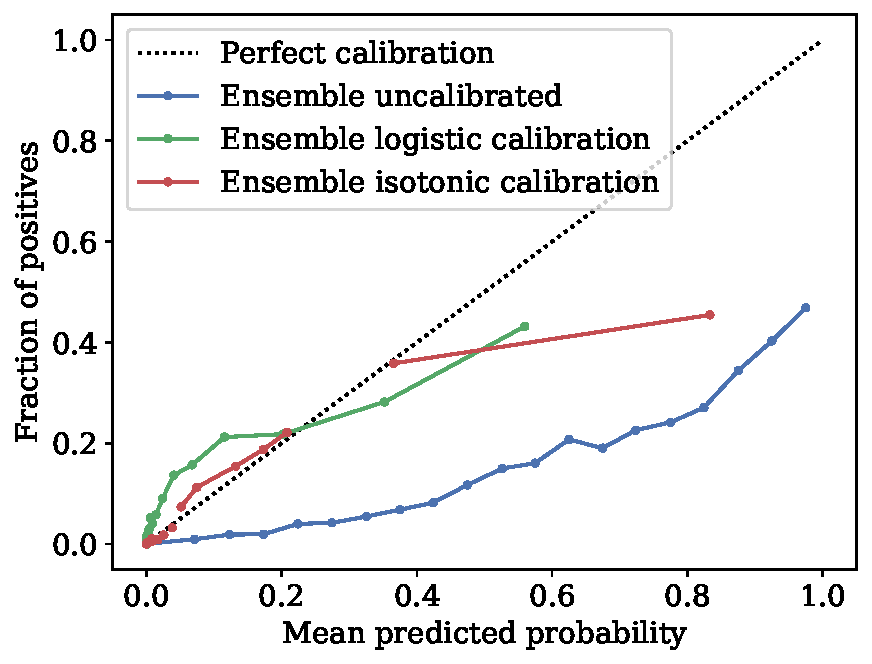
\includegraphics[width=1\columnwidth]{paper_retrospective_calibration_plots/calibration_curves_ensemble.pdf}
        % \caption{}
        % \label{fig_discussion:calibration_curve_ensemble_and_all_models_uncalibrated}
    \end{subfigure}    
    % \hfill
    \begin{subfigure}[c]{0.48\columnwidth}
        \centering
        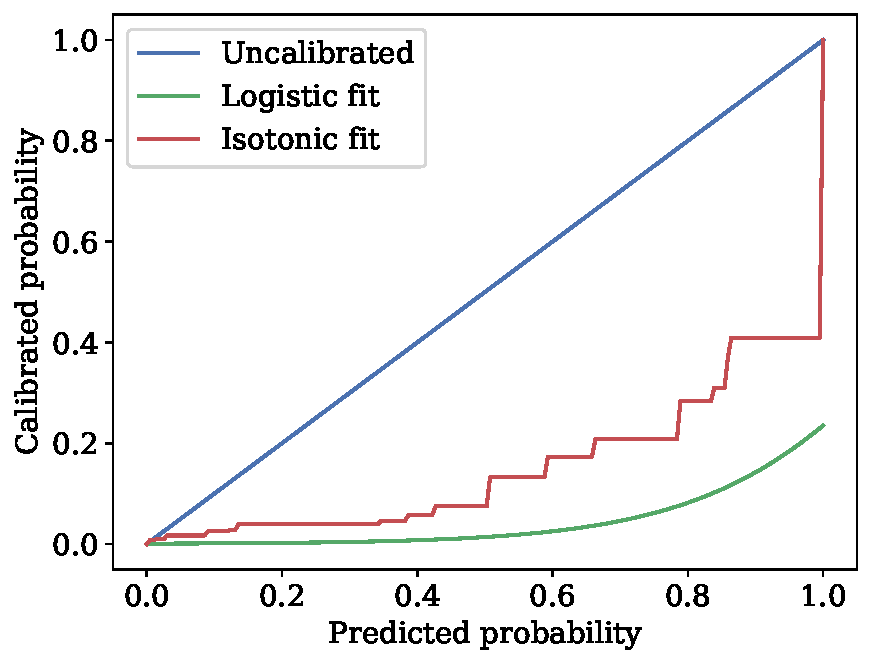
\includegraphics[width=1\columnwidth]{paper_retrospective_calibration_plots/calibration_fits_ensemble.pdf}
        % \caption{}
        % \label{fig_discussion:histogram_ensemble_and_single_model}
    \end{subfigure}    
    \caption[Calibration fits and curves for the stroke recognition ensemble using Platt-scaling and isotonic regression for calibration.]{ Calibration curves using sigmoid and isotonic calibration fits for the stroke recognition ensemble model (left) and the calibration fits (right) for the test set. We use the ensemble that achieved the median F1-score reported in \cref{tab_retrospective:table3-occlusion-analysis} and \cref{fig_retrospective:figure1-roc-curve}.}
    \label{fig_discussion:retrospective-paper-calibration-curve-sigmoid-isotonic}
\end{figure}    

Clinicians in intensive care units and emergency departments have been found to strongly agree that a singular focus on overall accuracy cannot ensure sustained use of and trust in a model \cite{tonekaboni_what_2019}. Clinicians expect an alert to present a prediction that aligns with patient status. Despite expert-agreed thresholds for when alerts should be triggered, however, many alerts may not be aligned since the unbalanced and ambiguous nature of many predictive problems in healthcare can lead to low predictive precision \parencite{umscheid_development_2015, cite14, cite15, wenstrup_retrospective_2023}. This can lead to alarm fatigue \parencite{embi_evaluating_2012} and can undermine the use and endorsement by clinicians of such systems \parencite{guidi_clinician_2015}. 
The expected precision of the stroke recognition ensemble of $24.9\%$ (95\% confidence interval $24.3-25.5\%)$ means it might be wrong three out of four times it predicts a positive. This unfortunately makes alarm fatigue likely among its potential users which might diminish it's real-world impact.

If the stroke recognition ensemble were to be deployed in a randomized controlled trial, such issues might be alleviated by incorporating the calibrated probabilities in the alerts presented to users. With calibrated probabilities, user would be able to discern between certain and uncertain model predictions or might be presented only with predictions that exceed a specific confidence level. Similar approaches have been suggested by clinicians and interviews indicate that predictive uncertainty is perceived as a sort of explanation that complements the prediction \cite{tonekaboni_what_2019}.


\begin{figure}
    \begin{subfigure}[c]{0.48\columnwidth}
        \centering
        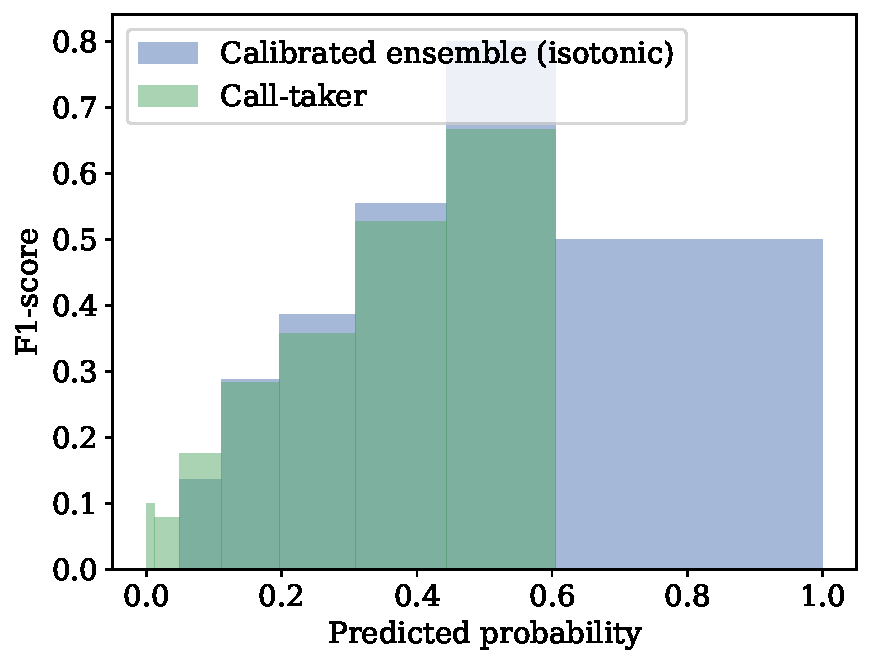
\includegraphics[width=1\columnwidth]{paper_retrospective_calibration_plots/f1_score_vs_predicted_probability_ensemble_calltaker}
        % \caption{}
        % \label{fig_discussion:calibration_curve_ensemble_and_all_models_uncalibrated}
    \end{subfigure}    
    % \hfill
    \begin{subfigure}[c]{0.48\columnwidth}
        \centering
        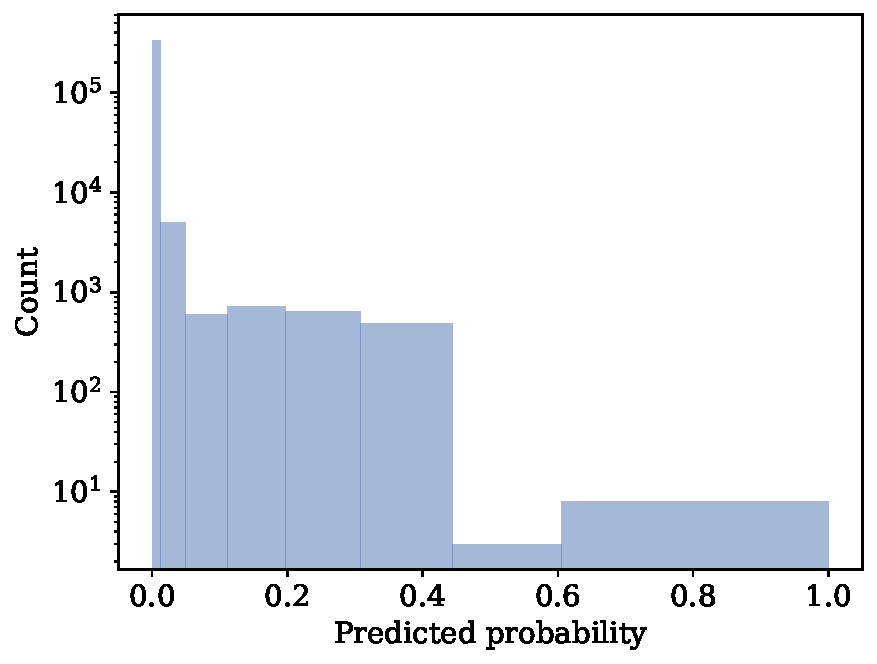
\includegraphics[width=1\columnwidth]{paper_retrospective_calibration_plots/predicted_probability_histogram.pdf}
        % \caption{}
        % \label{fig_discussion:histogram_ensemble_and_single_model}
    \end{subfigure}    
    \caption[Comparison of F1-score of stroke recognition ensemble and call-takers as function of predicted probability.]{ Comparison of the F1-score of the stroke recognition ensemble and call-takers. The F1-score is computed on subsets of the test dataset made by binning on the calibrated probabilities of the ensemble. We see that the relative performance improvement of the ensemble over call-takers is higher towards more certain predictions. We use the ensemble that achieved the median F1-score reported in \cref{tab_retrospective:table3-occlusion-analysis} and \cref{fig_retrospective:figure1-roc-curve}.}
    \label{fig_discussion:retrospective-paper-calibration-curve-sigmoid-isotonic}
\end{figure}    

Inspecting the 

\todo[inline]{Finish this sentence and analysis.}

Nevertheless, while correct calibration provides some explanation to the predictions, the actual value of the calibrated probabilities is still tied of the model's performance. By inspecting \cref{fig_discussion:retrospective-paper-calibration-curve-sigmoid-isotonic}, we can see that the logistic calibration shifts the predicted probabilities so far towards zero that the highest possible predicted probability is about 50\%. This means strokes can be predicted at best with a 50\% chance of being correct which limits the potential reduction in alarm fatigue. 

\todo[inline]{Finish this sentence and analysis.}

Making matters worse, the most certain model predictions are the ones that agree the most with call-taker judgment (see \cref{fig_discussion:retrospective-paper-fractional-agreement-vs-probability}). Hence, keeping the most certain predictions also means reducing the potential for changing call-taker.. Not really if when the model disagrees at low prob it is always right while when it disagrees at high prob it is always wrong (although unlikely and contrary to calibration - but that was done for the total set of predictions, not subgroups)


This highlights a problem where combining predictions with well-calibrated uncertainties may not be sufficient to ensure sustained use in practice.



% \lesstodo[inline]{Discuss the calibration of the stroke model and report calibration curve.}
% \lesstodo[inline]{Report the results of calibrating the stroke model using e.g. Platt scaling or Isotonic scaling.} % https://scikit-learn.org/stable/modules/calibration.html

% \lesstodo[inline]{Maybe mention MultiQT paper \parencite{havtorn_multiqt_2020}.}
